\section{Numerical details of obtaining dephasing rates}
\label{app:dephasing_numerics}

This section details the numerical procedure used to extract the dephasing rates in
Sec.~\ref{subsec:numerical_total_dephasing_rate}. The dynamics are
simulated with the full Hamiltonian $H_{\mathrm{full}}(\delta\Phi)$ represented in a
truncated oscillator (Fock) basis and evolved under the Lindblad master equation
\begin{align}
\dot{\rho}
&= -i\!\left[\,H_{\mathrm{full}}\big(\delta\Phi(t)\big),\ \rho\,\right]
+ \gamma_{b\downarrow}\,\mathcal{D}[b]\rho,
\label{eq:lindblad_full}
\end{align}
where $\mathcal{D}[b]\rho=b\rho b^\dagger-\tfrac{1}{2}\{b^\dagger b,\rho\}$.
\paragraph{Generation of $1/f$ noise.} Flux noise is incorporated through stochastic trajectories $\delta\Phi(t)$ whose spectrum
follows a $1/f$ power spectral density. For each trajectory, Eq.~\eqref{eq:lindblad_full}
is integrated to obtain $\rho(t)$, and all reported curves are computed from ensemble
averages of the corresponding observables. The noise realizations $\delta\Phi(t)$ are
generated using the frequency-domain synthesis method of Ref.~\cite{timmer1995generatingcolornoise}:
Fourier components are assigned random phases and Gaussian-distributed amplitudes with
variances proportional to the target $1/f$ spectrum, followed by an inverse Fourier
transform to obtain $\delta\Phi(t)$ in the time domain. Fig.~\ref{fig:psd} shows the
resulting power spectral densities for 100 representative trajectories. This ensemble size
is sufficient for the quantities of interest to converge, as indicated by the small error
bars in Fig.~\ref{fig:total_rate}(a) and Fig.~\ref{fig:relaxation_excitation_plot}(b).

\begin{figure}
    \centering
    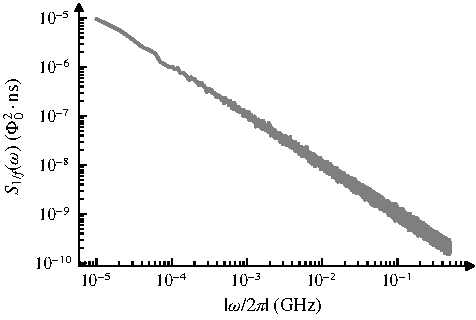
\includegraphics[width=\linewidth]{Appendix/noise_spectrum_plot.pdf}
    \caption{Power spectral density of $\delta\Phi(t)$ for 100 representative $1/f$ noise
    trajectories generated with the cutoffs specified below.}
    \label{fig:psd}
\end{figure}

The total simulated evolution time is $T\sim 10~\mu\mathrm{s}$, and the infrared cutoff
is set to $\omega_{\mathrm{IR}}/2\pi=10~\mathrm{kHz}$ (equivalently
$f_{\min}=10^{-5}\,\mathrm{GHz}$). This choice satisfies $f_{\min}\ll 1/T \approx 100~\mathrm{kHz}$,
capturing the relevant slow-noise dynamics within the simulated window while avoiding the
infrared divergence of an ideal $1/f$ spectrum. The ultraviolet cutoff is set to
$f_{\max}=1~\mathrm{GHz}$; the extracted dephasing rates are insensitive to further
increases of $f_{\max}$.

\paragraph{Extraction of dephasing time.} The states with enhanced dephasing discussed in main text are proxies for the corresponding Floquet states, as shown in Appendix~\ref{app:floquet}.
In the numerics, Floquet modes are labeled by their correspondence to bare states as
described in Appendix~\ref{app:numerics}. The two Floquet states used for the cavity
dephasing analysis in Sec.~\ref{subsec:numerical_total_dephasing_rate}
are denoted $\ket{\phi_{g,0}(t)}$ and $\ket{\phi_{g,1}(t)}$.

Relaxation and dephasing are extracted from dynamics evolving from two initial states. Relaxation is
characterized by preparing
\[
\rho(0)=\ket{\phi_{g,1}(0)}\!\bra{\phi_{g,1}(0)}
\]
and monitoring the return toward \(\ket{\phi_{g,0}(t)}\). Dephasing is characterized by preparing the equal superposition
\[
\rho(0)=\ket{+}\!\bra{+},
\qquad
\ket{+}=\frac{1}{\sqrt{2}}\Big(\ket{\phi_{g,0}(0)}+\ket{\phi_{g,1}(0)}\Big),
\]
and tracking the decay of the corresponding coherence. The relevant quantities are
\[
\mathrm{Tr}\!\left[\rho(t)\,P_{g,0}(t)\right]
\quad \text{and} \quad
\mathrm{Tr}\!\left[\rho(t)\,X(t)\right],
\]
where
\[
P_{g,0}(t)=\ket{\phi_{g,0}(t)}\!\bra{\phi_{g,0}(t)},
X(t)=\ket{\phi_{g,1}(t)}\!\bra{\phi_{g,0}(t)}+\mathrm{H.c.}
\]


Relaxation and dephasing times are obtained by fitting ensemble-averaged signals.
Specifically, $T_1$ is extracted from the rise of the ground-state population by fitting
$\mathrm{Tr}\!\left[P_{g,0}(t)\,\overline{\rho}(t)\right]$ to $1-e^{-t/T_1}$, where
$\overline{\rho}(t)$ denotes the ensemble-averaged density matrix over different flux noise trajectories. The coherence time $T_2$
is extracted from the decay of the superposition signal by fitting
$\mathrm{Tr}\!\left[P_{+}(t)\,\overline{\rho}(t)\right]$ to $e^{-t/T_2}$ (with the appropriate
normalization convention for the plotted data). The pure dephasing time then follows from
\begin{align}
\frac{1}{T_\phi}=\frac{1}{T_2}-\frac{1}{2T_1},
\end{align}
and we report the total dephasing rate as $\Gamma_{\phi,\mathrm{total}}=1/T_\phi$.
The data in Fig.~\ref{fig:total_rate} use the same system parameters and level truncations
as Appendix~\ref{app:numerics}. Unless otherwise stated, the fitting windows are
$1~\mu\mathrm{s}$ for $T_1$ and $5~\mu\mathrm{s}$ for $T_2$; extending these windows
does not change the extracted rates.